\documentclass{standalone}

\usepackage{tikz}
\usetikzlibrary{shapes.geometric, arrows}

\tikzstyle{start} = [rectangle, rounded corners, minimum width=2cm, minimum height=1cm,text centered, draw=black, fill=red!30]
\tikzstyle{stop} = [rectangle, rounded corners, minimum width=2cm, minimum height=1cm,text centered, draw=black, fill=blue!30]

\tikzstyle{io} = [trapezium, trapezium left angle=70, trapezium right angle=110, minimum width=2cm, minimum height=1cm, text centered, draw=black, fill=blue!30]
\tikzstyle{process} = [rectangle, minimum width=1cm, minimum height=1cm, text centered, draw=black, fill=orange!30]
\tikzstyle{classifier} = [rectangle, minimum width=2cm, minimum height=1cm, text centered, draw=black, fill=green!30]
\tikzstyle{decision} = [diamond, minimum width=2cm, minimum height=1cm, text centered, draw=black, fill=green!30]

\tikzstyle{arrow} = [thick,->,>=stealth]

\begin{document}
	
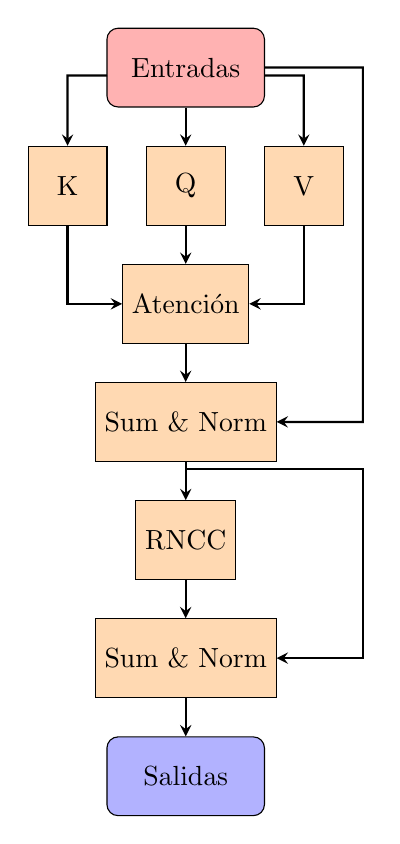
\begin{tikzpicture}[node distance=1.5cm]
\node (start) [start, text width=1.5cm] {Entradas};
%\node (enc) [process, below of=start] {Codificador};
\node (Q) [process, below of=start] {Q};
\node (K) [process, left of=Q] {K};
\node (V) [process, right of=Q] {V};
\node (Att) [process, below of=Q] {Atención};
\node (SN) [process, below of=Att] {Sum \& Norm};
\node (FCN) [process, below of=SN] {RNCC};
\node (SN2) [process, below of=FCN] {Sum \& Norm};

\node (stop) [stop, below of=SN2] {Salidas};


%\node (outs) [startstop, left of=dec, xshift=-1.3cm, text width=2cm] {Salidas anteriores};
%\node (clas) [classifier, below of=dec] {Clasificador};

%\node (out) [stop, below of=clas, text width=2cm] {Salida siguiente};

%\node (pro1) [process, below of=in1] {Process 1};
%\node (dec1) [decision, below of=pro1, yshift=-0.5cm] {Decision 1};

\draw [arrow] (start) -- (Q);
\draw [arrow] (start) -- node {} ++(-1cm, -0.1cm) -| (K);
\draw [arrow] (start) -- node {} ++(+1cm, -0.1cm) -| (V);

\draw [arrow] (K) |- node {} ++(0cm, -1.5cm) -- (Att);
\draw [arrow] (Q) -- (Att);
\draw [arrow] (V) |- node {} ++(0cm, -1.5cm) -- (Att);

\draw [arrow] (Att) -- (SN);
\draw [arrow] (SN) -- (FCN);
\draw [arrow] (FCN) -- (SN2);

\draw [arrow] (SN2) -- (stop);

\draw [arrow] (start) -- node {} ++(+2.25cm, 0cm) -| node {} ++(0cm, -4.5cm) -- (SN);

\draw [arrow] (SN) |- node {} ++(+2.25cm, -0.6cm) -| node {} ++(0cm, -2cm) |- (SN2);

%\draw [arrow] (enc) -- (dec);
%\draw [arrow] (dec) -- (clas);
%\draw [arrow] (clas) -- (out);

%\draw [arrow] (outs) -- (dec);

%\draw [arrow] (in1) -- (pro1);
%\draw [arrow] (pro1) -- (dec1);

\end{tikzpicture}

\end{document}